\documentclass[lettersize,journal]{IEEEtran}
\usepackage{amsmath,amsfonts}
\usepackage{algorithmic}
\usepackage{array}
\usepackage[caption=false,font=normalsize,labelfont=sf,textfont=sf]{subfig}
% \usepackage{cite}
\usepackage{textcomp}
\usepackage[ngerman]{babel} % Dokumentensprache auf Deutsch setze
\usepackage{stfloats}
\usepackage{url}
\usepackage{verbatim}
\usepackage{graphicx}
\usepackage{balance}
\usepackage[acronym]{glossaries}
\usepackage{subcaption}
\usepackage{hyperref}
\usepackage{cleveref}
\usepackage[style=ieee,hyperref]{biblatex}
\addbibresource{references.bib}
\usepackage{etoolbox}
\AtBeginBibliography{\footnotesize}
\DefineBibliographyStrings{german}{
  andothers = {et al.},
  and = {und}
}

% Benutzerdefinierter Zitierbefehl, um Autor, Titel, Jahr und Zitiernummer anzuzeigen und zu verlinken
\DeclareCiteCommand{\customtextcite}
  {\usebibmacro{prenote}}
  {\usebibmacro{citeindex}%
   \printnames{labelname}%
   \setunit{\addcomma\space}%
   \printfield{title}%
   \setunit{\addcomma\space}%
   \printfield{year}%
   \setunit{\addspace}%
   \printtext[bibhyperref]{[\printfield{labelnumber}]}}
  {\multicitedelim}
  {\usebibmacro{postnote}}


\makeglossaries

% Define acronyms
\newacronym{adam}{ADAM}{Adaptive Moment Estimation}
\newacronym{arima}{ARIMA}{Autoregressive Integrated Moving Average
% (z.Dt. Autoregressiver integrierter gleitender Durchschnitt)
}
\newacronym{garch}{GARCH}{Generalised Autoregressive Conditional Hetero-Skedasticity Model 
% (z.Dt. Verallgemeinerte autoregressive bedingte Hetero-Skedastizität)
}
\newacronym{lstm}{LSTM}{Long Short-Term Memory}
\newacronym{cnn}{CNN}{Convolutional Neural Network}
\newacronym{rnn}{RNN}{Recurrent Neural Network}
\newacronym{llm}{LLM}{Large Language Model}
\newacronym{gbt}{GBT}{Gradient Boosted Trees}
\newacronym{xai}{XAI}{Explainable AI}
\newacronym{eda}{EDA}{Explorative Datenanalyse}
\newacronym{ki}{KI}{Künstlichen Intelligenz}

\begin{document}

% EXAMPLES

% \begin{figure*}[h]
%   \centering
%   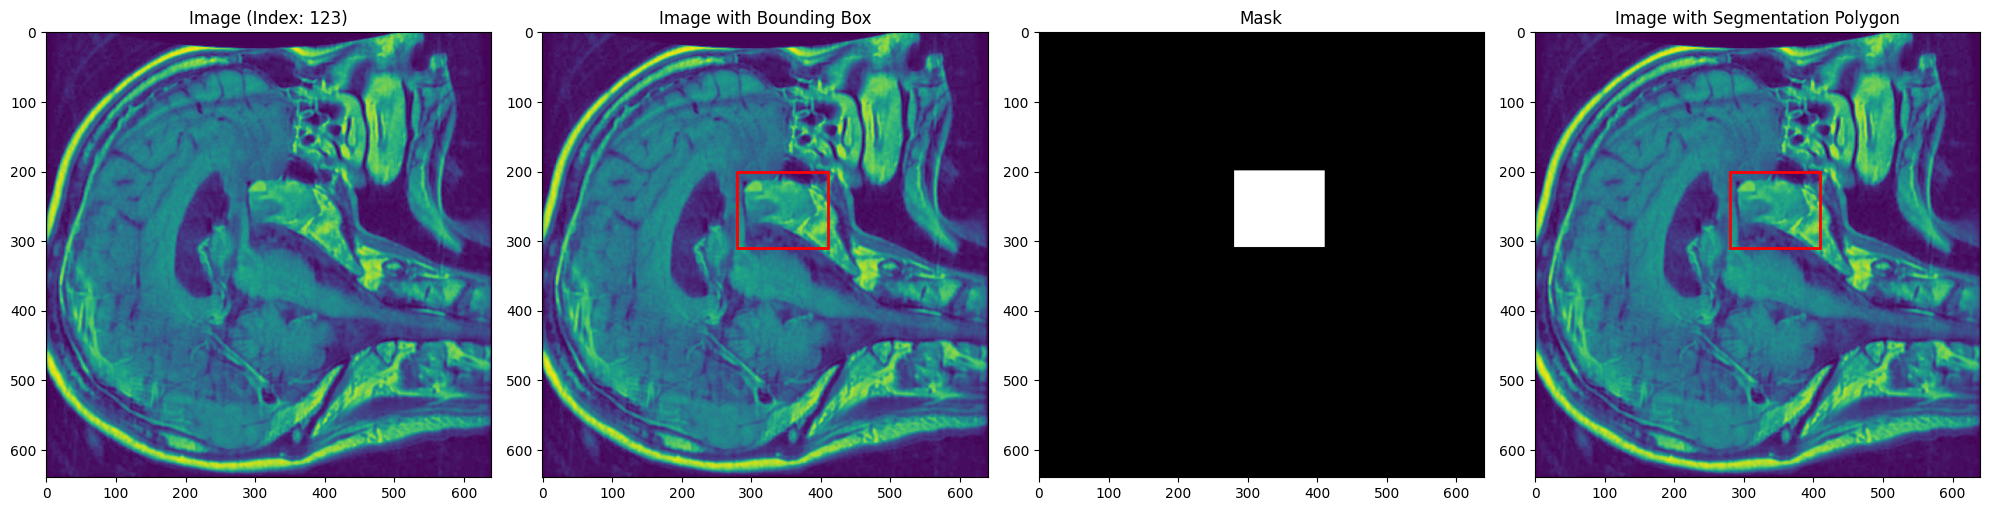
\includegraphics[width=\textwidth]{images/du_image_and_mask.png}
%   \caption{Plot of a sample image from the data set, the image with bounding box, the corresponding mask and the visualization of the polygon to show that the polygon does not contain any further useful information compared to the bounding box.}
%   \label{fig:da_image_and_mask}
% \end{figure*}

% \begin{figure*}[h]
%   \centering
%   \subfloat{\label{fig:image5}%
%       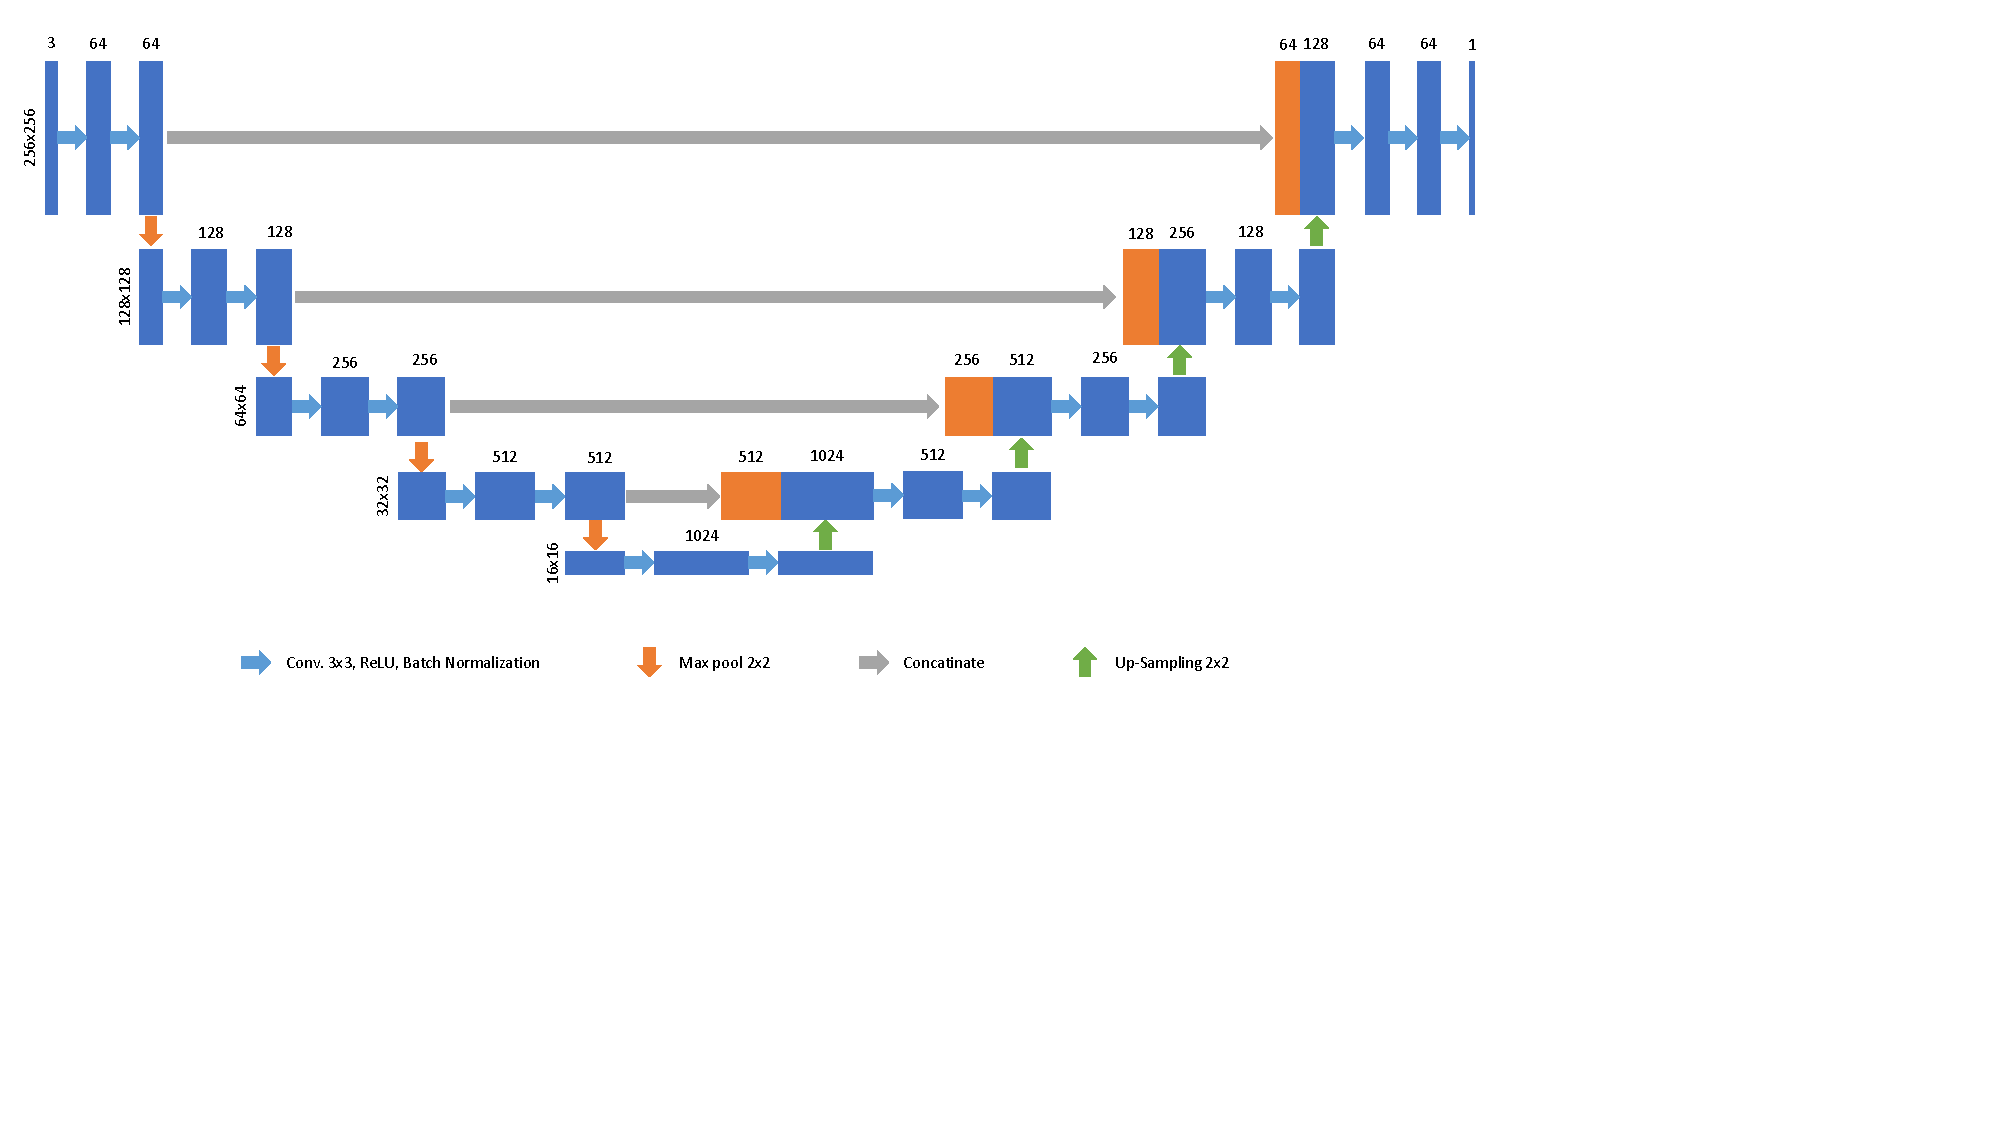
\includegraphics[width=0.45\textwidth]{images/Selfdesigned_unet.pdf}} \quad
%   \subfloat{\label{fig:image6}%
%       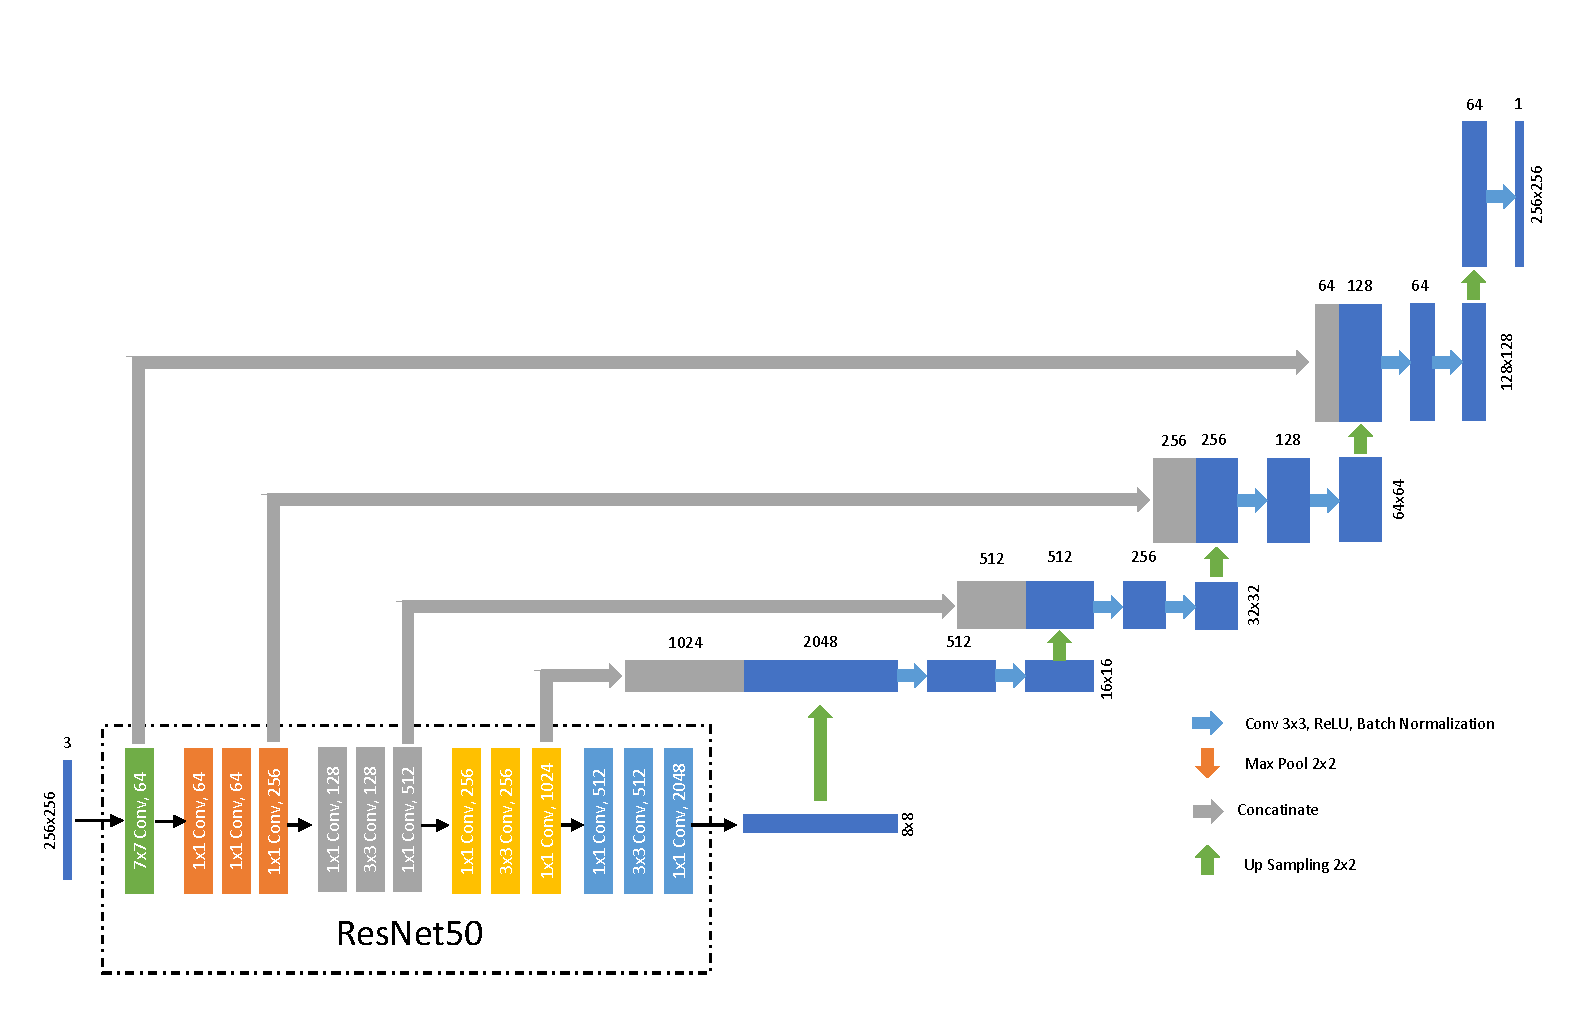
\includegraphics[width=0.45\textwidth]{images/Pretrained_unet-cropped.pdf}}
%   \caption{Model architectures of the self-designed UNet and the UNet with pre-trained ResNet50 backbone}
%   \label{fig:models}
% \end{figure*}

% Acronym \gls{adam} 
% Formula terms \( y \) and \( \hat{y} \). Equation:

% \begin{equation}
% {L} = - \left( y \log(\hat{y}) + (1 - y) \log(1 - \hat{y}) \right)
% \end{equation}

% In alignment to the definitions above we used the following formulas to calculate the evaluation metrics of our models with \( y_i \) and \( \hat{y}_i \) representing the actual and predicted values for the \(i\)-th pixel, respectively, and the total number of pixels denoted by \( N \):
% \begin{itemize}
%   \item \textbf{Accuracy} is the ratio of correctly predicted pixels to the total number of pixels:
%   \begin{equation}
%   \text{Accuracy} = \frac{1}{N} \sum_{i=1}^{N} \left( y_i \hat{y}_i + (1 - y_i) (1 - \hat{y}_i) \right)
%   \end{equation}
% \end{itemize}


\title{Datenanalyse, Hypothesentests und Entwicklung eines prädiktiven Deep Learning Modells für Auftragseingänge durch kontextbewusste Multi-Source-Datenfusion}
% Development of a Predictive Deep Learning Model for Order Intake through Context-Aware Multi-Source Data Fusion

\author{Jakob Müller
\thanks{Diese Arbeit ist als Studienarbeit am DHBW Center for Advanced Studies in Heilbronn entstanden. Die hier zum Ausdruck gebrachten Meinungen sind ausschließlich die des Autors. Es wird keine Garantie übernommen. Der Benutzer trägt das gesamte Risiko.
  %This work is created as a student research project at the Cooperative State University Baden-Württemberg Center for Advanced Studies at Heilbronn. The opinions expressed here are entirely that of the author. No warranty is expressed or implied. User assumes all risk.
  }}
\markboth{DHBW Center for Advanced Studies, Prof. Dr. Dirk Reichardt, July~2024}%
{Entwicklung eines prädiktiven Deep Learning Modells für Auftragseingänge durch kontextbewusste Multi-Source-Datenfusion}



\maketitle



\begin{abstract}
  Diese Arbeit behandelt die Identifikation von Mustern und Zusammenhängen, speziell Korrelation, Kovarianz und Granger-Kausalität (Präzedenz), zwischen dem Auftragseingang und unternehmensinternen Vertriebsdaten, wie Kundenaccounts, Verkaufschancen und Aufträgen, sowie externen Daten wie Wirtschaftsindikatoren, Trenddaten (Aufrufe in Suchmaschinen wie Google), Nachrichten und Aktienkursen inklusive der Entwicklung prädiktiver Deep-Learning-Modelle für den Auftragseingang unter Anwendung des Konzepts der Multi-Source-Datenfusion, um die Genauigkeit und Erklärbarkeit der Prognosen für zukünftige Auftragseingänge und damit die Geschäftssituation zu erhöhen. Dafür werden zunächst unternehmensinterne mit externen Daten zu einem multimodalen Datensatz integriert. Anschließend wird eine explorativ-deskriptive und diagnostische Datenanalyse durchgeführt, um Hypothesen und Zusammenhänge im Datensatz mit dem Auftragseingang zu identifizieren und mit statistischen Methoden, darunter Korrelations-, Kovarianz- und Granger-Kausalitätstests, zu prüfen. Darauf aufbauend werden prädiktive Deep Learning Modelle unterschiedlicher Architekturen für die Auftragseingangsvorhersage entwickelt und verglichen und dabei das Konzept der kontextbewussten Multi-Source-Datenfusion angewendet. Aufbauend auf aktuellen Arbeiten zu Transformer Modellen, Deep-Learning-Architekturen und der Fusion mehrerer Datenquellen werden Large Language Models und Text Embeddings genutzt, um Textdaten mit unternehmensinternen und externen Daten zu integrieren, die Änderungen in der wirtschaftlichen Entwicklung und den Marktbedingungen widerspiegeln. Ziel ist es, die Leistungsfähigkeit dieser Technologien auf die Vorhersage von Auftragseingängen zu übertragen und somit die Genauigkeit der Vorhersage und die Entscheidungsfindung in Unternehmen zu verbessern.
\end{abstract}

\begin{IEEEkeywords}
Auftragseingagnsvorhersage, Explorative Datenanalyse, Prädiktive Modelle, Deep Learning, Transformer Modelle, Multi-Source-Datenfusion, Large Language Models, Text Embeddings, Wirtschaftsindikatoren.
\end{IEEEkeywords}


\section{Einführung}
\IEEEPARstart{M}{it} der schnellen Entwicklung der künstlichen Intelligenz und der Emergenz digitaler Ökonomien erhält die globale Wirtschaft zunehmenden Aufschwung. Wirtschaftsindikatoren wie Aktienkurse reflektieren Änderungen in der wirtschaftlichen Entwicklung und in Marktbedingungen. 

\subsection*{Problemstellung}
Datengetriebene Prognose- und Entscheidungsmodelle sind in der modernen Wirtschaft wichtig, um Unternehmensentscheidungen in Bezug auf Produktion, Lagerhaltung und Ressourcenplanung zu informieren. % Diese Zeile nicht in Anmeldung übernehmen
Auftragseingangsvorhersagen ermöglichen es Unternehmen, zukünftige Nachfrage präzise zu prognostizieren, Ressourcen effizient zu planen und strategische Entscheidungen zu optimieren, um Wettbewerbsvorteile zu sichern. 
Viele Unternehmen verlassen sich bezüglich ihrer operativen und strategischen Entscheidungen vor allem auf intuitive Vorhersagen von Markttrends und Nachfrageschwankungen durch Experten. In Zeiten von Volatilität und schnellem Wandel ist die Geschäftssituationsanalyse und die Präzision von Vorhersagen kritisch für den Erfolg, um frühzeitig neue Situationen zu erkennen und effektive Maßnahmen zu treffen.
\subsection*{Ziel der Arbeit}
Ziel dieser Arbeit ist die Identifikation von Mustern und Zusammenhängen zwischen dem Auftragseingang und internen Vertriebsdaten, wie Kundenaccounts, Verkaufschancen und Aufträgen, sowie externen Daten wie Wirtschaftsindikatoren, Trenddaten (Aufrufe in Suchmaschinen), Nachrichten und Aktienkursen, um die Genauigkeit und Erklärbarkeit der Prognosen für zukünftige Auftragseingänge und damit der Geschäftssituation zu erhöhen.


\subsection*{Forschungsfrage und Hypothesen}
Die Arbeit beschäftigt sich im Kern mit der Frage, welche Muster und Zusammenhänge zwischen dem Auftragseingang und den genannten internen und externen Daten bestehen, wie die Auftragslage vorausschauend sinnvoll eingeschätzt und wie die zukünftige Entwicklung des Auftragseingangs vorhergesagt werden kann. Die Ergebnisse werden auf Basis der folgenden Hypothesen analysiert, die auf den gegebenen Anwendungsfall zur Auftragseingangsvorhersage limitiert sind:
\begin{enumerate}
  \item \textbf{Relevanz interner und externer Daten}: Die Integration von externen Trend-, Wirtschafts- und Ereignisdaten neben den unternehmensinternen Daten verbessert signifikant die Vorhersagegenauigkeit von Auftragseingängen gegenüber Modellen, die ausschließlich interne oder externe Daten verwenden.
  \item \textbf{Pragmatismus komplexer Machine Learning Modelle für die Auftragseingangsvorhersage}: Die Modellkomplexität und Genauigkeit stehen in einem optimalen Verhältnis, sodass komplexere Modelle, welche maschinelles Lernen einsetzen, genauer sind als vereinfachte statistische Modelle und die intuitive Vorhersage von Auftragseingängen durch Experten, ohne dabei an praktischer Anwendbarkeit zu verlieren, wenn Erklärbarkeit durch XAI-Techniken gewährleistet wird.
  \item \textbf{Relevanz und Effektivität von Multi-Source-Datenfusionsmechanismen für die Auftragseingangsvorhersage}: Durch die Übertragung dieser Konzepte auf die Vorhersage von Auftragseingängen kann die Genauigkeit und Verlässlichkeit der Prognosen verbessert werden.
  \item Weitere noch auszuarbeitende Hypothesen zum Zusammenhang von Daten mit dem Auftragseingang, speziell auch zu externen Einflüssen
\end{enumerate}

\section*{Methodik}
Nach einer vorläufigen Literaturrecherche zur Thematik wird zunächst der OECD-Datensatz erstellt und beschafft. Dieser Datensatz bildet die Grundlage für die erste Phase der Analysen und Experimente. Im Anschluss daran werden spezifische Funktionen zur Prüfung der Hypothesen entwickelt und unmittelbar anhand des OECD-Datensatzes getestet.

Darauf folgt die Implementierung des Codes für die Modellexperimente. Diese Experimente umfassen alle Schritte der Modellentwicklung, vom Modelltraining bis hin zur Evaluation. Wie die Analysen werden auch die initialen Modellexperimente zuerst ausschließlich mit dem OECD-Datensatz durchgeführt. In der nächsten Phase wird der Datensatz erweitert und die Analysen und Modellexperimente auf den so entstandenen Datensätzen durchgeführt, um alle Experimente anschließend zu vergleichen und dabei die entdeckten Zusammenhänge und die Modellperformance zu erforschen.

Der erweiterte Datensatz entsteht durch die Integration unternehmensinterner und externer Datenquellen, um ein umfassendes multimodales Datenset zu erstellen. Datenquellen umfassen neben der API des OECDs das unternehmensinterne Salesforce-System mit diversen Vertriebsdaten sowie weitere externe APIs wie Google Trends, NewsAPI und Yahoo Finance. Programmiert wird in Python mit Jupyter Notebook unter Verwendung der nachfolgend genannten wesentlichen Bibliotheken.

Insgesamt gliedert sich die systematischen Vorgehensweise zur Erkennung von Mustern und Zusammenhänge mit dem Auftragseingang sowie der Entwicklung von Vorhersagemodellen in drei Phasen: (1) Explorativ-deskriptive Datenanalyse, (2) diagnostische Analyse und Hypothesentests (3) Modellentwicklung, -validierung und -erklärung.
\subsection{Explorativ-deskriptive Datenanalyse (EDA)}
Die explorativ-deskriptive Datenanalyse bildet die Grundlage der Hypothesenbildung. Zunächst werden die internen Unternehmensdaten und externen Wirtschaftsdaten aggregiert und visuell sowie statistisch analysiert. Ziel der EDA ist es, die Bedeutung und Struktur der Daten zu verstehen und Hypothesen zu bilden.
\subsection{Diagnostische Analyse und Hypothesentests}
Auf Basis der Ergebnisse der EDA werden spezifische Hypothesen formuliert. Diese Hypothesen zielen darauf ab, die Beziehungen zwischen den verschiedenen Datensätzen und dem Auftragseingang darzustellen und zu testen. Konkret geht es um die Beziehungstypen Korrelation, Kovarianz und Granger-Kausalität (bzw. Präzedenz). Ein Beispiel für eine solche Hypothese könnte sein: \glqq Ein Anstieg des Bruttoinlandsprodukts führt zu einem proportionalen Anstieg der Auftragseingänge.\grqq \space Für das Testen der Hypothesen werden Korrelations-, Kovarianz- und Granger-Kausalitätstest angewendet. Dafür soll die Bibliothek statsmodels genutzt werden.
\subsection{Modellentwicklung und -erklärung}
Basierend auf den validierten Hypothesen werden prädiktive Modelle entwickelt. Hierfür stehen fortschrittliche Machine Learning-Algorithmen wie \gls{lstm}-Netzwerke, \glspl{cnn} und Transformer-Modelle zur Auswahl, die zumindest in einem neuronalen Netz mit Fully-Connected-, LSTM-, CNN- und Transformer-Encodern kombiniert und in einem Fully-Connected-Decoder zusammengeführt werden sollen. Die Modelle werden darauf trainiert, auf Basis der Werte der Feature-Zeitreihen der letzten 12 Monate die zukünftigen Auftragseingänge der folgenden 12 Monate vorherzusagen, dann mit geeigenten Metriken evaluiert und mit Baseline-Modellen verglichen. Für die Modellentwicklung werden die Bibliotheken Keras und Scikit-Learn verwendet.

\subsection{Modellerklärung}
Abschließend wird die Erklärbarkeit der Modelle durch \gls{xai} Techniken geprüft, um die Entscheidungen der Modelle nachvollziehbarer zu machen. Genutzt wird dafür die Bibliothek Shap.

\section{Vorgehensweise}
\subsection*{Literaturrecherche} Zunächst erfolgt eine systematische Literaturrecherche zur Untersuchung von bestehenden Ansätzen und Methoden für die Analyse und Prognose von Finanzdaten in ähnlichen Anwendungsbereichen unter Verwendung von Datenbanken (IEEE Explore, Google Scholar, Researchgate, arXiv), Verlagen (Springer, Wiley, De Gruyter) und spezifischen Journals für Data Science, KI und den Finanzbereich (The Economist, New Scientist, The Economic Journal, American Economic Journal), um ein fundiertes Verständnis des Themenbereichs zu erlangen, bestehende Modelle und Methoden zu verstehen und Forschungslücken zu identifizieren.
\subsection*{Datenerhebung und Datenintegration} Hier werden relevante Unternehmensdaten (z. B. Verkaufszahlen, Kundenfeedback) gesammelt und passende externe Datenquellen (z. B. Wirtschaftsindikatoren, Trenddaten, Nachrichtenkanäle) identifiziert. 
\subsection*{Datenexploration und -vorberarbeitung} In diesem Schritt werden Verständnis, Bereinigung und Aufbereitung der erhobenen Daten für die nachfolgende Analyse und Modellierung erzielt, um die Datenqualität und damit die Effektivität der Analysen und Modelle zu optimieren. 
\subsection*{Explorativ-deskriptive und diagnostische Datenanalyse} Anschließend erfolgt die Analyse der erhobenen Daten auf Muster und Zusammenhänge mit dem Auftragseingang zur Formulierung und zum Testen von Hypothesen, um das Verständnis der Daten zu vertiefen. Methodisch können deskriptive Statistik, Korrelationsanalysen und Hypothesentests eingesetzt werden. Um Hypothesen über Muster und Zusammenhänge im gegebenen Datensatz zu generieren, werden typische statistische Darstellungen und Kennwerte verwendet. 
\subsection*{Modellentwicklung} Danach erfolgen Entwicklung, Auswahl und Test verschiedener maschineller Lernalgorithmen und Modelle (auszuwählen und ggf. in Hypothesen integrieren) zur Erstellung von Modellen für die Vorhersage von Auftragseingängen sowie die Auswahl des besten Modells.
% Verschiedene Modelle können unterschiedlich gut für die Vorhersage geeignet sein (wann sind welche Modelle besonders erfolgreich, speziell für diese Anwendung? Warum braucht es komplexe Modelle?); durch die Evaluation mehrerer Ansätze kann das optimale Modell gefunden werden.
\subsection*{Test und Evaluation} In diesem Rahmen werden geeignete Metriken für die Genauigkeit des Modells festgelegt und Vorhersagen anhand von Testdaten der letzten Zeiträume durchgeführt sowie mit bestehenden Prognosen zur Bewertung und Verbesserung der Prognosefähigkeit verglichen.
\subsection*{Modellerklärung und Interpretation} Zur Interpretation der Modellentscheidungen und zur Transparenzsteigerung werden XAI-Techniken (Explainable AI) genutzt, um Vertrauen in das Modell zu schaffen und Einsichten für Entscheidungsträger zu geben.
\subsection*{Erweiterung der Datenbasis} Nachdem diese Schritte zunächst für den Datensatz mit den OECD-Daten durchgeführt wurden, sollen dann weitere Datensätze durch die Ergänzung mit Daten aus den oben genannten Quellen erstellt und die entwickelten Analysen und Modellexperimente darauf angewendet und die Ergebnisse mit jeweils allen Datensätzen verglichen werden. Um die News-Daten in die Vorhersage aufzunehmen, werden diese zunächst nach Suchbegriffen von NewsAPI (oder, falls Zugriff besteht, auch von NewscatcherAPI) abgerufen und nach Monat ihrer Veröffentlichung geordnet. Dann werden für jeden Monat mithilfe eines Large Language Models eine Zusammenfassung der Artikel des jeweiligen Monats mit den für die Auftragseingagnsvorhersage relevanten Themen und Aspekten erstellt. Für jeden Monat wird dann zusätzlich eine Zusammenfassung der Zusammenfassungen der Vormonate erstellt, um auch die Einflüsse aus der Vergangenheit abzudecken. Die Embeddingd beider Zusammenfassungen, die dann für jeden Monat erstellt sind, werden dann in das Modell integriert.
\subsection*{Zusammenfassung, Diskussion und Ausblick} Abschließend folgt die Zusammenfassung und kritische Reflexion der Ergebnisse und Ableitung erster unternehmerischer Handlungsempfehlungen auf Basis der Daten sowie die Formulierung von Handlungsempfehlungen und Perspektiven für zukünftige Forschung und Entwicklung.

\section{Zeitplan}
Ein erster Stand für die Integration der OECD-Daten und der historischen Daten des Auftragseingangs sowie der Korrelations-, Kovarianz- und Granger-Kausalitätsanalysen und der Modellentwicklung-, -evaluation und -erklärung ist entwickelt. Es folgt die Prüfung und das Refinement dieses Prozesses sowie die Erweiterung des Datensatzes und die systematische Durchführung und Auswertung der Modelle mit allen erweiterten Datensätzen bis Mitte Dezember. Ein erster Stand der Arbeit ist bis Mitte Januar zu erwarten. Der Abgabetermin ist der 22.02.25.



\section{Gliederungsentwurf}

\begin{enumerate}
  \item Abstract / Zusammenfassung
  \item Executive Summary
  \item Einleitung
  \begin{enumerate}
    \item Schlüsselbegriffe
    \item Trends und Entwicklungen in den Bereichen Finanzen, Controlling und Business Data Analytics
    \item Revolutionierung der Finanzindustrie durch Big Data udn fortgeschrittene Analysen und Transformation von Geschäftsmodellen, Entscheidungsprozessen und Strategien (bezogen auf Unternehmen) durch Risikokontrolle, Marktanalyse, Sentimentanalyse und Deep Learning
    \item Erfolgreiche Datenanalyse für das Controlling
    \item Forschungsgegenstand
    \item Motivation und Forschungsinteresse
    \item Ziel der Arbeit
    \item Forschungsfrage
    \item Hypothesen
    \item Methodik und Vorgehensweise
    \begin{enumerate}
      \item Darstellung der Themen für den Grundlagenteil
      \item Literaturrecherche
      \item Datenerhebung
      \item Datenexploration und –vorverarbeitung
      \item Datenanalyse
      \item Modellentwicklung
      \item Evaluation
      \item Modellerklärung und Interpretation
    \end{enumerate}
  \end{enumerate}
  \item Grundlagen
  \begin{enumerate}
    \item Kurz: Controlling (Definition, Ziele, Kernaspekte)
    \item Optional: Wirtschaftspolitik und Wirtschaftsindikatoren, Theorie des Effizienten Marktes, Informationen im Wirtschaftssystem
    \item Optional: Operations Research, Entscheidungsfindung, Eintscheidungsinformation und Strategie. Wie werden Vorhersagen und Analysen zum aktuellen Stand der Geschäftssituation, wie etwa in Form von Zusammenfassungen von News oder auch anderen Texten aus der Branche, genutzt, um optimale strategische und Operative Entscheidungen in der Unternehmensplanung (z.B. Supply Chain Management und Controlling) zu treffen?
    \item Kurz: Sales (Ziele, Prozess und Daten, Erfolgsmessung, Beitrag von AE-Prognosen)
    \item Data Science (Definition, Ziele, Kernaspekte) und Data Science Prozess (CRISP-DM)
    \item Descriptive, Diagnostic, Predictive und Prescriptive Analytics
    \item Kurz: Statistische Methoden der Explorativen Datenanalyse: Plots, Kennzahlen, Hypothesentests, Korrelationsanalyse
    \item Fokus: Neuronale Netze (Architekturen und Schichten,Trainingskonzepte inklusive Mathematik: Aufbau, Forward Propagation, Backpropagation, Gradient Descent, Optimierer)
    \item Fokus: Explainable AI
    \item Fokus: Evaluationsmetriken
  \end{enumerate}
  \item Durchführung
  \begin{enumerate}
    \item Vorgehensweise
    \begin{enumerate} 
      \item Literaturrecherche
      \item Datenerhebung 
      \begin{enumerate}
        \item Beschreibung der Datenquellen
        \item Darstellung der Datenintegration
      \end{enumerate}
      \item Datenexploration und –vorverarbeitung
      \item Datenanalyse
      \item Modellentwicklung
      \item Evaluation
      \item Modellerklärung und Interpretation
    \end{enumerate}
    \item Ergebnisse
    \begin{enumerate}
      \item Darstellung und Interpretation der Kausalitätstests.
      \item Beantwortung der Frage, welche Indikatoren mit dem Auftragseingang korrelieren bzw. im Sinne der Tests eine zeitliche Ursächlichkeit indizieren.
      \item Darstellung und Interpretation der Evaluationsergebnisse für jedes Modell und für jeden Datensatz
      \item Beantwortung der Frage, welche Datensätze die Vorhersage des Auftragseingangs im Vergleich zur ausschließlichen Verwendung von Wirtschaftsindikatoren verbessern.
      \item Beantwortung der Frage, ob Deep Learning-Modelle für die Vorhersage des Modells sinnvoll sind basierend auf ihrer Performance im Vergleich zu einfachen Modellen (Linear Regression und XGBoost)
    \end{enumerate}
  \end{enumerate}
  \item Zusammenfassung
  \begin{enumerate}
    \item Zusammenfassung der Ergebnisse
    \item Kritische Würdigung und Diskussion
    \item Ausblick und zukünftige Arbeiten
  \end{enumerate}
\end{enumerate}



\section{Forschungsstand}
Die Vorhersage von Aktienkursen ist ein bekannter Anwendungsfall, der künstliche Intelligenz und maschinelles Lernen nutzt, um zukünftige Kursentwicklungen basierend auf historischen Daten und Marktindikatoren zu prognostizieren. Diese Modelle berücksichtigen eine Vielzahl von Variablen, darunter Wechselkurse, Änderungen in steuerpolitischen Regelungen, Marktstimmung und makroökonomische Bedingungen, um präzise Vorhersagen zu treffen \cite{mo2024backgroundawaremultisourcefusionfinancial}. Ähnlich wie bei der Aktienkursvorhersage ist die Vorhersage von Auftragseingängen für Unternehmen von entscheidender Bedeutung, da sie die Grundlage für strategische und operative Entscheidungen bildet.

Datengetriebene Prognose- und Entscheidungsmodelle sind in der modernen Wirtschaft wichtig, um Unternehmensentscheidungen in Bezug auf Produktion, Lagerhaltung und Ressourcenplanung zu informieren. Auftragseingangsvorhersagen ermöglichen es Unternehmen, zukünftige Nachfrage präzise zu prognostizieren, Ressourcen effizient zu planen und strategische Entscheidungen zu optimieren, um Wettbewerbsvorteile zu sichern. 
Viele Unternehmen verlassen sich bezüglich ihrer operativen und strategischen Entscheidungen vor allem auf intuitive Vorhersagen von Markttrends und Nachfrageschwankungen durch Experten. In Zeiten von Volatilität und schnellem Wandel ist die Präzision dieser Vorhersagen kritisch für den Erfolg.
Ziel der Arbeit ist die Identifikation relevanter Muster und Zusammenhänge zwischen Unternehmensdaten und externen Daten und dem Auftragseingang zur Erhöhung der Genauigkeit und Erklärbarkeit der Prognosen für zukünftige Auftragseingänge

Wirtschafts- und Finanzprognosen, wie Aktienkurs- oder Auftragseingagnsvorhersagen, werden durch Faktoren wie Wechselkurse, Steuerpolitik, Marktstimmung und makroökonomische Bedingungen beeinflusst \cite{Zhang2018ImprovinStockMarketPrediction}. Der Kapitalmarkt ist nach der Theorie des Effizienten Marktes sogar dadurch charakterisiert, dass er alle verfügbaren Informationen reflektiert \cite{Fama1970EfficientMarkets}. Infolgedessen sind die Analyse und die Vorhersage solcher Variablen mit erheblichen Herausforderungen verbunden. Sowohl die quantitative Analyse, die Faktoren wie Aktienkurse, Einkommen und Bilanzen nutzt, als auch die qualitative Analyse, die das Management, Produkte und Strategien beleuchtet, sind wichtig, um erfolgreiche Investmentstrategien am Kapitalmarkt zu entwickeln und daher ist es auch sinnvoll, umfassende Informationen inklusive quantitativer Zahlen und qualitativer Beschreibungen zu sammeln, um Trends am Kapitalmarkt vorherzusagen \cite{Zhang2018ImprovinStockMarketPrediction}. Weil Unternehmen im Allgemeinen Teil des Wirtschaftssystems sind, das der Kapitalmarkt abbildet, gelten diese Überlegungen auch für die Vorhersage anderer wesentlicher Finanzdaten wie den Auftragseingang.

Traditionelle Vorhersagemodelle wie ARIMA und Exponential Smoothing zeigen ihre Grenzen insbesondere in hochvolatilen und komplexen Umgebungen \cite{Wasserbacher2022machinelearningfpa}. Fortschrittlichere Modelle wie \gls{lstm}, \glspl{cnn}, Transformer und Embedding Transformations bieten jedoch vielversprechende Ansätze zur Verbesserung der Vorhersagegenauigkeit. Diese Modelle ermöglichen es, komplexe Muster und Beziehungen in großen und heterogenen Datensätzen zu erkennen \cite{mo2024backgroundawaremultisourcefusionfinancial}.

Aktuelle Herausforderungen beinhalten die Integration und Verarbeitung vielfältiger Datenquellen, die Handhabung von Informationslücken in Daten, die die tatsächliche Situation nicht vollständig beschreiben, wie es wirtschaftlichen Anwendungen der Fall ist, sowie die Skalierbarkeit und Interpretierbarkeit der Modelle. Ziel dieser Arbeit ist es weiterhin, diese Herausforderungen durch die Entwicklung eines prädiktiven Deep Learning Modells für Auftragseingänge zu adressieren, das kontextbewusste Multi-Source-Datenfusion nutzt und so in der Lage ist, wesentlich mehr Informationen zur allgemeinen wirtschaftlichen Situation über die Fusion mit verschiedenen Textquellen und der Anwendung von \glspl{llm} und Embedding Transformations abzubilden.

Durch die Übertragung dieser Konzepte auf die Vorhersage von Auftragseingängen kann die Genauigkeit und Verlässlichkeit der Prognosen verbessert werden. Die Integration verschiedener Datenquellen wie Unternehmensdaten und Wirtschaftsindikatoren sowie die Anwendung moderner Lernverfahren hat das Potenzial, die Vorhersagekraft wesentlich zu verbessern und bietet daher ein relevantes und zeitgemäßes Forschungsthema. 


% Relevanz, Herausforderungen, Forschungsstand, Forschungsbedarf, Ziel der Arbeit und wie die Herausforderungen adressiert werden, Forschungsfrage, Hypothesen, Warum bieten die in der Arbeit behandelten Themen das Potential, die Herausforderungen zu lösen und warum ist das ein relevantes und zeitgemäßes Forschungsthema?


\section{Vorläufige Literaturrecherche}
Zum aktuellen Zeitpunkt wurde eine kompakte Literaturrecherche durchgeführt, um ein erstes Verständnis für das Thema zu erzielen und Forschungslücken zu identifizieren. Nachfolgend ist die Methodik beschrieben, bevor im Abschnitt \ref{sec:VerwandteArbeiten} die Ergebnisse in Form einer Darstellung relevanter Literatur enthalten sind.

\subsection{Schlüsselbegriffe}
Zunächst wurden folgende zum Thema passende Schlüsselbegriffe definiert:

\begin{itemize}
  \item Sales Predictions, Sales forecasting, predicitve models for sales
  \item Machine Learning, predictive analytics, data analytics, pattern recognition, hypothesis testing, data mining, explorative data analysis
  \item Finance, controlling, business analytics, economic forecasting, business predictions, enterprise data, external sources
  \item Economic indicators, sales data, stock market, stock movement
  \item Data preprocessing, data integration, data management, data collection, data analysis
  \item Performance metrics, evaluation, explainable artificial intelligence, xai, interpretability techniques
  \item Future trends, developments, market trends, techniques, algorithms
  \item Systematic review, literature review, empirical study, development, implementation
\end{itemize}


\subsection{Ein- und Ausschlusskriterien}
Anschließend wurden folgende Ein- und Ausschlusskriterien definiert:

\begin{itemize}
  \item Sprache: Studien, die in Englisch verfasst sind, da dies die vorherrschende Wissenschaftssprache ist und die breiteste Zugänglichkeit gewährleistet.
  \item Publikationszeitraum: Studien, die seit 2018 veröffentlicht wurden, um sicherzustellen, dass die in der Analyse verwendeten Technologien und Methoden aktuell sind. Ausnahmen sind Artikel, die grundlegende und bedeutende Konzepte beschreiben.
  \item Studientyp
  \begin{itemize}
    \item Empirische Studien, die quantitative Analysemethoden verwenden und keine Editorials, Kommentare oder Meinungsartikel.
    \item Fallstudien, die spezifische Beispiele für die Anwendung von Data Science und KI in der Vorhersage von Auftragseingängen darstellen.
		\item Übersichtsarbeiten und Meta-Analysen, die einen Überblick über den aktuellen Forschungsstand zu Vorhersagen im Finanzbereich geben.
		\item Keine Patente und kommerziellen Werbematerialien, die nicht einer wissenschaftlichen Peer-Review unterzogen wurden.
  \end{itemize}
  \item Thematische Relevanz
  \begin{itemize}
    \item Studien, die sich explizit mit der Entwicklung von prädiktiven Modellen für Auftragseingänge oder ähnliche wirtschaftliche Prognoseaufgaben oder Aufgaben, die für die Entwicklung eines prädiktiven Modells nützlich sein können, oder der Identifikation von Mustern und Zusammenhängen durch Datenanalyse beschäftigen.
    \item Studien, Artikel und Bücher, die sich mit Methoden der Statistik, Datenanalyse, Data Science und KI beschäftigen, die für den Gegenstand der Arbeit relevant sind.
    \item Keine Studien, die keine Verbindung zwischen ihren Forschungsergebnissen und Mustern, Zusammenhängen oder der Vorhersage von Auftragseingängen auf Basis interner und externer Datenquellen herstellen können oder zu denen sich keine herstellen lässt.
		\item Studien, die maschinelles Lernen und KI-Methoden in der Vorhersage von Unternehmenskennzahlen verwenden.
		\item Forschungsarbeiten, die die Integration von Unternehmensdaten und externen Daten wie Konjunkturindikatoren untersuchen.
		\item Artikel, die sich mit Explainable AI (XAI) im Kontext von Prognosemodellen beschäftigen.
  \end{itemize}
\end{itemize}

\subsection{Literatursuche}
Anschließend wurden die Bibliotheken von ArXiv, Google Scholar, Science Direct und IEEE Explore durchsucht. Dafür wurden die oben genannten Suchbegriffe zu Sucheingaben kombiniert. So wurden entsprechend der Ein- und Ausschlusskriterien 61 relevante Suchergebnisse gefunden, von denen die fünf relevantesten in diesem Exposé aufgenommen wurden und im Abschnit \ref{sec:VerwandteArbeiten} dargestellt sind.

Die so durchgeführte Literaturrecherche wird im Rahmen der Studienarbeit noch erweitert.

\section{Grundlagenliteratur}
\begin{itemize}
  \item Zu Statistik: \customtextcite{BambergBaurKrapp+2022} und \customtextcite{Bourier2022BeschreibendeStatistik}. 
  \item Zu Data Mining: \customtextcite{olson2023deskriptives}. 
  \item Zu Statsitik, Data Mining und maschinelles Lernen: \customtextcite{YANG201967} und \customtextcite{Liu2016}. 
  \item Zu Konzepten der \gls{ki}: \customtextcite{Goerz2021HandbuchKI}
  \item Zu mathematischen Grundlagen der Data Science: \customtextcite{knoblauch2024mathematik}
\end{itemize}


\section{Verwandte Arbeiten} \label{sec:VerwandteArbeiten}

Für die Entwicklung eines prädiktiven Modells nutzt diese Arbeit Erkenntnisse und Konzepte der Arbeit von \customtextcite{mo2024backgroundawaremultisourcefusionfinancial} und behandelt darauf aufbauend das Thema der Vorhersage von Unternehmensfinanzkennzahlen, speziell den Auftragseingang. Der Artikel beschreibt einen neuen Mechanismus zur Vorhersage von Trends, speziell im Bereich Finanzen und Wirtschaft am Anwendungsfall der Aktienkursvorhersage, der ein \gls{llm}, insbesondere das MacBERT-Modell, einsetzt, um Informationen aus Texten wie Aktienkursbewertungen und Berichten aus der Politik zu nutzen und diese mit Aktienpreisdaten zu integrieren. Diese kombinierten Merkmale werden dann für das Training neuronaler Netze mit unterschiedlichen Architekturen eingesetzt, um umfassende Marktanalysen zu ermöglichen. Die Architektur des Konzepts ist in Abbildung \ref{fig:backgroundawaremultisourcefusion} dargestellt. Experimente zeigen, dass der Mechanismus die Genauigkeit von Aktienbewegungsvorhersagen verbessert, was auf die Einbeziehung der Berichte über das Sprachmodell zurückzuführen ist.
Der Artikel liefert der Arbeit Modellierungs- und Trainingskonzepte sowie Mechanismen für die Integration unterschiedlicher Datenquellen, Anreize für die Behandlung der Erklärbarkeit von Vorhersagen und Implementierungsstrategien.

\begin{figure*}[h]
  \centering
  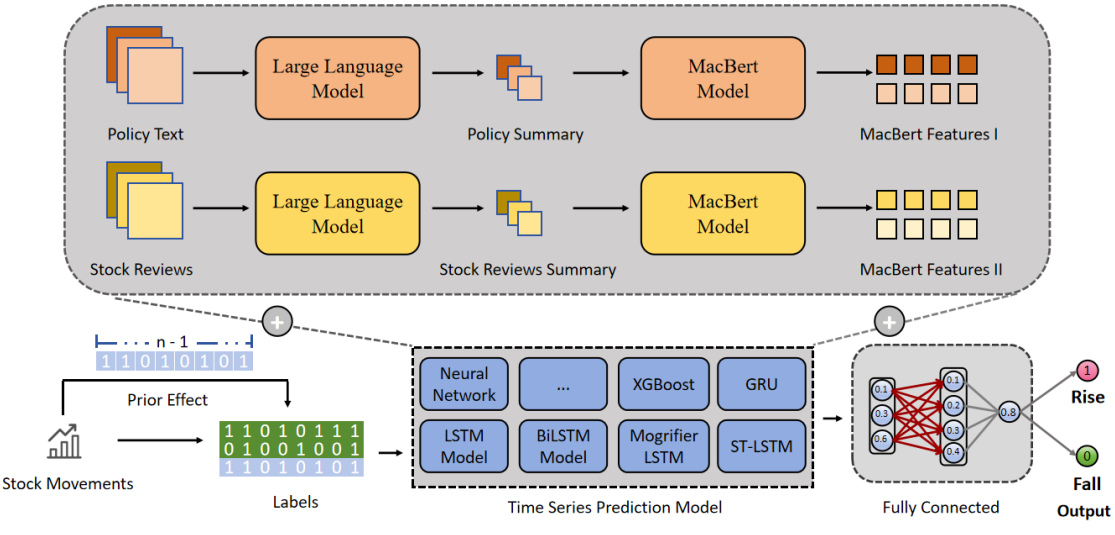
\includegraphics[width=\textwidth]{images/Architektur Background-Aware Multi-Source Fusion.png}
  \caption{Modellarchitektur mit Implementierung kontextbewusster Multi-Source Datenfusion aus \cite{mo2024backgroundawaremultisourcefusionfinancial}}
  \label{fig:backgroundawaremultisourcefusion}
\end{figure*}

Der Artikel von \customtextcite{Wasserbacher2022machinelearningfpa} bietet für die Arbeit eine umfassende Einführung in den Einsatz von maschinellem Lernen für Finanzprognosen, Planung und Analyse (FP\&A). Dabei wird auch thematisiert, dass die Anwendung von maschinellem Lernen für Planungs- und Ressourcenallokationsaufgaben im Kontrast zu Prognoseaufgaben problematisch sein kann, da diese Aufgaben kausale Inferenz erfordern, was schwierig zu modellieren ist. Im Artikel wird ein Framework vorgestellt, um kausale Zusammenhänge zu behandeln und die Auswirkungen der Anwendung von Prognosen zu schätzen.

Der Artikel von \customtextcite{Benidis2022DlTimeSeriesForecastingTutorialLiteratureSurvey} bietet eine umfassende Einführung und einen Überblick über den EInsatz von Deep-Learning-Methoden zur Zeitreihenvorhersage mit einer Einführung in die Vorhersage von Zeitreihen, einer detaillierten Dartstellung der wichtigsten Elemente moderner tiefer Lernmodelle und einer Übersicht über den aktuellen Stand der Forschung und Anwendung im Bereich der Zeitreihenvorhersage. Dabei werden gängige Modelle und Techniken vorgestellt, darunter \glspl{rnn}, \glspl{cnn} und Transformers, sowie State Space Models und probabilistische Ansätze.

Der Artikel von \customtextcite{Cheriyan2018IntelligentSalesPredictionUsingMachineLearningTechniques} beschäftigt sich ähnlich wie diese Arbeit mit der Entwicklung eines intelligenten Vorhersagesystems für Verkaufszahlen mittels maschineller Lerntechniken. Ziel ist es ebenfalls, zuverlässige Verkaufsprognosen zu erstellen, die Unternehmen bei der Ressourcenplanung und Entscheidungsfindung unterstützen. Der Artikel beschreibt verschiedene Techniken und Modelle, die zur Verbesserung der Effektivität von Verkaufsprognosen eingesetzt werden können. Die Evalutation verschiedener Modelle im Rahmen der Studie ergibt, dass der Gradient Boost Algorithm die höchste Vorhersagegenauigkeit bietet. Im Unterschied zu dieser Arbeit werden ausschließlich interne quantitative Daten für Modellierung und Vorhersage verwendet. Interessant ist sowohl, dass der \gls{gbt} Algorithums eine Vorhersagegenauigkeit von 98 \% erreicht und somit auch zu prüfen, wie diese Methode für den im Rahmen dieser Arbeit gegebenen Anwendungsfall funktioniert.











%\section[Methods]{Dataset}

% \section[Method]{Methoden}
%( Method, Approach** (incl. theory), Development method (data, model architecture, hyperparameters, ...) )

% \section[Results]{Results}

% \section{Conclusion}




\balance

\begin{tiny} % oder \scriptsize, \tiny je nach gewünschter Größe
  \printbibliography
\end{tiny}

% \bibliographystyle{IEEEtran}
% \bibliography{references}

% \begin{thebibliography}{1} %Example of a Citation: According to a well-known study \cite{ams}, the mathematical typesetting is crucial for clear presentation.

% \bibitem{ams}
% {\it{Mathematics into Type}}, American Mathematical Society. Online available: 

% \bibitem{oxford}
% T.W. Chaundy, P.R. Barrett and C. Batey, {\it{The Printing of Mathematics}}, Oxford University Press. London, 1954.

% \bibitem{lacomp}{\it{The \LaTeX Companion}}, by F. Mittelbach and M. Goossens

% \end{thebibliography}


% \printglossaries


\end{document}

